\begin{frame}
	\frametitle{}
	\Background[1] 
	\begin{center}
	{ {\Huge 总~复~习 (2学时)}}
	\end{center}    
\end{frame}

\begin{frame} 
      \frametitle{四个方程}
      \begin{enumerate}
          \item 基础:常微分方程基本解法 (15\%)
          \item 三大偏微分方程 (40\%)
          \item 一个薛定谔方程 (含氢原子) (45\%)
      \end{enumerate}
      \begin{center}
           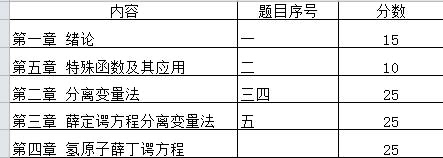
\includegraphics[width=0.8\textwidth]{figs/2022-05-10-13-48-04.png}
      \end{center}
\end{frame}

\begin{frame} [label=current] 
 \frametitle{每个方程的主要内容}
 \begin{enumerate}
     \item 方程的建立
     \item 方程的求解技巧
     \item 解的特性~固有解的正交性和平方积~叠加解的系数
     \item 应用~解的物理意义~求复杂积分,...
 \end{enumerate}
      
\end{frame}


\section{1. 常微分方程基本解法}

\subsection{一阶常微分方程}

\begin{frame}
\frametitle{1. 衰减与增长模型}
\begin{exampleblock} {例1、	放射性衰减模型}
	\begin{equation*}
	\frac{du}{dt}	= - ru, ~~~~ u(t_0) = u_0
	\end{equation*}
	\end{exampleblock} 	
	\alert{解:} 分离变量
	\begin{align*}
		\frac{du}{u} &= - rdt\\
		\ln u &=-rt+C\\
		u(t)&=C'exp(-rt)	
	\end{align*}
	初始条件定系数:
	\begin{equation*}
		u(t)=u_0 exp(-rt)
	\end{equation*}
    {\color{red}{[X]}} 半衰期 
\end{frame}

\begin{frame}
	\begin{exampleblock} {例2、	人口增长的逻辑斯蒂模型}
	\begin{equation*}
		\frac{d u}{d t}=r u (1-u/K)
	\end{equation*}
	\end{exampleblock} 	
	\alert{解:} 分离变量:
	\begin{align*}
		&(\frac{1}{K-u}+\frac{1}{u} ) d u =r d t \\
		&-\ln (K-u)+\ln u =r t+C \\
		&u(t) = \frac{K}{1+ \exp (-r t-C)}	\\
	\end{align*}	
\end{frame}

\begin{frame}
        \begin{exampleblock} {非齐次问题}
        \begin{equation*}
            y'+py=f(x)
        \end{equation*}
        \end{exampleblock}
        \alert{解、} 衰减模型齐次方程有解:\\
        \begin{center}
            $y=C_0 exp(-px)$
        \end{center} 
        {\color{red}{[X]}} 常系数变易, 设非齐次方程的解为\\ 
        \begin{center}
            $y(x) =C(x) exp(-px)$
        \end{center} 
        代入原方程,解得系数多项式:
            \[C(x) = \int exp(px) f (x)dx + C\]
        代回,原方程有解 \[  y(x)=C exp(-px)+exp(-px) \int exp(px)f(x)dx \]
    \end{frame}

\subsection{二阶常微分方程}

\begin{frame}
	\frametitle{振动模型}
	\begin{exampleblock} {例 3、建立简谐振动微分方程并求解}	
	\begin{center}
		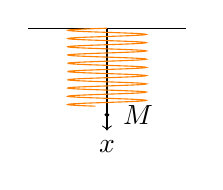
\begin{tikzpicture} [scale=0.5]
	\draw  (-2,0) -- (2,0) node[below] {};
	\draw [->] (0,0) -- (0,-2.6) node[below] {$x$};	
	\draw [orange, domain=0:-1.98, samples=200] plot({sin(\x r *30)},\x);
	\draw [fill, black, circle] (0,-2.2) circle(0.3ex) node[right] {$M$};
    \end{tikzpicture} 
	\end{center}
	\end{exampleblock}
	\alert{解、} 牛顿第二定律建立方程:\\
	\begin{equation*}
		-k x = F = Ma = M\frac{d ^2 x}{d t^2} 
	\end{equation*}
	\begin{equation*}
		\frac{d ^2 x}{d t^2} +\frac{k}{M} x =0, 
	\end{equation*}	
\end{frame}

\begin{frame}	
	整理,得:
	$\displaystyle \begin{cases}
	\dfrac{d ^2 x}{d t^2} +\omega ^2 x = 0	\\
	x(t)\left |_{t=0}  =x_0  \right. ,  \quad  \dfrac{dx}{dt} \left |_{t=0}  =0 \right.      	
	\end{cases}$\\ \vspace*{0.6em}
	{\color{red}{[X]}}辅助方程 : $u^2+\omega ^2=0$, 有两虚根:$u_{1, 2} =\pm i\omega$  \\
    方程通解: \[x(t)=C_1 \cos \omega t +C_2 \sin \omega t \]   	
	代入初始条件得解: \[x(t)=x_0 \cos \omega t \] 
\end{frame}

\begin{frame}
	\begin{exampleblock} {*阻尼振动-一阶项的物理意义}
	\begin{equation*}
		\frac{d^2 u}{d t^2} +2\varepsilon \frac{d u}{dt} +\omega ^2 u = 0 ,  ~~~ (\varepsilon < \omega)   
	\end{equation*}
	\end{exampleblock} 
	\alert{解、} {\color{red}{[X]}} 消一阶项! 令 $\displaystyle  u(t)= exp(-\varepsilon t) v(t) $,  代回原方程, 整理得: 
	\begin{equation*}
		\frac{d^2 v}{d t^2} +(\omega ^2 - \varepsilon ^2) u = 0,  ~~~ (\varepsilon < \omega)   
	\end{equation*}
    令 $k^2 =\omega ^2 - \varepsilon ^2 $, 得简谐振动微分方程标准型, 得解
	\begin{equation*}
		v(t)=C_1 \cos k t +C_2 \sin k t 
	\end{equation*}
	代回,方程得解: 
	\begin{equation*}
		u(t)= exp(-\varepsilon t) [ C_1 \cos \sqrt{\omega ^2 - \varepsilon ^2} t +C_2 \sin \sqrt{\omega ^2 - \varepsilon ^2} t] 
	\end{equation*}	
\end{frame}

\begin{frame}
	\begin{exampleblock} {*受迫振动-自由项的物理意义}
	\begin{equation*}
		\frac{d^2 u}{d t^2} + \omega ^2 u = p  \sin \omega_0 t
	\end{equation*}
	\end{exampleblock}
	\alert{解、} 齐次方程有解:
	\begin{equation*}
		u(t)=C_1 \cos \omega t +C_2 \sin \omega t 
	\end{equation*}
	设非齐次方程有特解:{\color{red}{[?]}} 为什么这么设
	\[  u(t) =C_0 \sin \omega_0 t  \]
	代回原方程, 得系数:
	\begin{align*}
		C_0 & = \frac{p}{\omega^2-\omega_{0} ^2 }
	\end{align*}
	原方程得解: \[ u(t)= C_1 \cos \omega t +C_2 \sin \omega t+ \frac{p}{\omega^2-\omega_{0} ^2 } \sin (\omega_0 t) \] 
\end{frame}

\begin{frame}
    \frametitle{变系数问题二例}
     变系数的物理含义
        \begin{exampleblock} {例 4、欧拉方程}
        \begin{equation*}
            x^2 \frac{d^2 y}{d x^2} +x \frac{d y}{d x} +n^2 y =0 
        \end{equation*}     
        \end{exampleblock}	
        \alert{解、}  令 $x=exp(t) , t=ln x $,代回方程,转化为常系数方程:
        \begin{equation*}
            \frac{d^2 y}{d t^2}  +n^2 y =0 
        \end{equation*}     
        是振动模型,有解:\[ 	y(t)=C_1 \cos n t +C_2 \sin n t \]
        原方程得解:
        \begin{equation*}
            y(x)=C_1 \cos (n \ln x) +C_2 \sin (n \ln x)
        \end{equation*}   
\end{frame}
\begin{frame}
        \begin{exampleblock} {欧拉方程的变型-1}
        \begin{equation*}
            x^2 \frac{d^2 y}{d x^2} +2x \frac{d y}{d x} -n(n+1) y =0 
        \end{equation*}     
        \end{exampleblock}
        \alert{解、} 	令 $x=exp(t) , (t=ln x) $, 代回,原方程可转化常系数方程:
        \begin{equation*}
            \frac{d^2 y}{d t^2}  +\frac{dy}{dt}-n(n+1) y =0 
        \end{equation*}     
        特征方程有两相异实根,方程的解为:
        \begin{equation*}
            y(t)=C_1 \exp (nt) +C_2 \exp (-(n+1) t)
        \end{equation*}  
        代回 t=ln x, 方程得解:
        \begin{equation*}
            y(x)=C_1 x^n +C_2 x^{-(n+1) }
        \end{equation*}  
\end{frame}

\begin{frame}
          \frametitle{}
          \begin{exampleblock} {欧拉方程的变型-2}
            \begin{equation*}
             x^2 \frac{d^2 y}{d x^2} +2x \frac{d y}{d x} -n^2 y =0    
            \end{equation*}     
            \end{exampleblock}
            \begin{exampleblock} {欧拉方程的变型-3}
            \begin{equation*}
            x^2 \frac{d^2 y}{d x^2} +2x \frac{d y}{d x} +(n\pi)^2 y =0 
             \end{equation*}     
            \end{exampleblock}   

\end{frame}
\begin{frame}
        \begin{exampleblock} {例 5、n 阶厄米方程}
        \begin{equation*}
            \frac{d^2 y}{d x^2} -2x \frac{d y}{d x} +2n y =0 
        \end{equation*}     
        \end{exampleblock}	
        \alert{解、} 设方程有级数解 
        \begin{equation*}
            y=\sum_{k=0}^{\infty} c_k x^k
        \end{equation*}     
        求导,对齐脚标, 代回原方程,$\cdots $ \\
        ~~ \\       
        {\Huge \hspace*{4em} \color{red}{[X]} 必须会}
\end{frame}

\subsection{傳里叶变换}

\begin{frame}
    \frametitle{傳里叶级数与变换}
        三角式: \\ \vspace{0.3em}
        { $\displaystyle f(x) =\dfrac{a_0}{2} +\sum_{n=1}^{\infty}  \left(  a_n \cos~ \frac{n\pi}{l} x +  b_n \sin~ \frac{n\pi}{l} x  \right) $ }\\	
        { $\displaystyle a_n =\frac{1}{l}  \int_{-l}^{l}  f(x )   \cos~ \frac{n\pi}{l} x dx, \quad a_n =\frac{2}{l}  \int_{0}^{l}  f(x )   \cos~ \frac{n\pi}{l} x dx  $ }\\	
        { $\displaystyle b_n =\frac{1}{l}  \int_{-l}^{l}  f(x )   \sin~ \frac{n\pi}{l} x dx, \quad b_n =\frac{2}{l}  \int_{0}^{l}  f(x )   \sin~ \frac{n\pi}{l} x dx   $ }\\	\vspace{0.6em}
        复数式:\\ \vspace{0.3em}
        {$\displaystyle f(x) =\sum_{n=-\infty}^{+\infty}  c_n e^{i\omega_n x} \qquad $  (不连续),   $ \qquad f(x) = \int_{-\infty} ^{+\infty} G(\omega) e^{i \omega x} d \omega $ (连续)}\\	
        {$\displaystyle c_n =\frac{1}{2l}  \int_{-l}^{l}  f(x)    e^{-i\omega_n x}  dx  $, $ \hspace*{6em} G(\omega) = \frac{1}{2\pi}\int_{-\infty} ^{+\infty} f(x) e^{-i \omega x} d x $  } \\
\end{frame}

\begin{frame}
      \frametitle{}
      对称式:\\ \vspace{0.3em}
      {$\displaystyle f(x) = \frac{1}{\sqrt{2\pi}}\int_{-\infty} ^{+\infty} G(\omega) e^{i \omega x} d \omega $}\\	
      {$\displaystyle G(\omega) = \frac{1}{\sqrt{2\pi}}\int_{-\infty} ^{+\infty} f(x) e^{-i \omega x} d x $  } \\ \vspace{0.6em}

      量子形式:\\ \vspace{0.3em}
      {$\displaystyle \psi(x) = \frac{1}{\sqrt{2\pi \hbar}}\int_{-\infty} ^{+\infty} c(p_x) e^{\frac{i}{\hbar} p_x x} d p_x $}\\	
      {$\displaystyle c(p_x) = \frac{1}{\sqrt{2\pi \hbar}}\int_{-\infty} ^{+\infty} \psi(x) e^{-\frac{i}{\hbar} p_x x} d x $  } \\
\end{frame}
\begin{frame}
    * 物理意义: 找到一组正交基,任意平滑函数都可以在这组正交基上展开. 
    \begin{exampleblock} {试求$\sin nx, \cos nx, e^{i\omega x}$ 的如下平方积}
    ~~\\
    \[ \begin{aligned}
            &\int_{-l} ^{l} \left| \sin \frac{n\pi x}{l} \right|^2 dx = l \\
            &\int_{-l} ^{l} \left| \cos \frac{n\pi x}{l} \right|^2 dx = l \\
            &\int_{-l} ^{l} \left| e^{i \dfrac{n\pi}{l} x} \right|^2  dx = 2l \\
            &\int_{-\infty} ^{+\infty} \left| e^{i \omega x} \right|^2  dx = 2\pi \\
    \end{aligned}\]
    \end{exampleblock}	
    * 平方积对应傳里叶公式前的系数
\end{frame}

\begin{frame}
    \begin{exampleblock} {试证明$\sin nx, \cos nx, e^{i\omega x}$ 的如下正交性 ($n \not = m $)}
    ~~\\
    \[ \begin{aligned}
            &\int_{-l} ^{l} \sin \frac{n\pi x}{l} \sin \frac{m\pi x}{l}  dx = 0 \\
            &\int_{-l} ^{l} \cos \frac{n\pi x}{l} \cos \frac{m\pi x}{l}  dx = 0 \\
            &\int_{-l} ^{l} e^{-i \dfrac{n\pi}{l} x} e^{i \dfrac{m\pi}{l} x}   dx = 0 \\
            &\int_{-\infty} ^{+\infty}  e^{-i \omega_n x} e^{i \omega_{m} x}   dx = 0 \\
    \end{aligned}\]
    \end{exampleblock}
    * 正交性是求函数具体展开式的关键	
\end{frame}

\section{2. 三大偏微分方程}


\subsection{波动导方程}

\begin{frame}
	\frametitle{波动方程的建立}	
    \alert{解:} 建立坐标系,  取任意微元ds, 临近拉力$T_1, T_2$:\\
	水平:{ $T_2\cos \alpha _2=T_1\cos \alpha _1=T_0$ }  \\   
	竖直:{$T_2\sin \alpha _2-T_1\sin \alpha _1=ma=\rho ds~ u_{tt} $}   \\   
	有~:{ $T_0(\tan \alpha _2-\tan \alpha _1)=\rho ds ~u_{tt}$ }   \\   \vspace{0.3 em}
    \hspace{1cm}$T_0[u_x(x+dx,t)-u_x(x,t)]=\rho dx ~u_{tt}$  \\   \vspace{0.6 em}
	\hspace{1cm}$\displaystyle \frac{T_0}{\rho}\times\frac{u_x(x+dx,t)-u_x(x,t)}{dx}=u_{tt}$ \\ \vspace{0.3 em}
	\Tips (1)斜率就是一阶导,(2)小角度条件下,$ds \simeq dx$, 整理,得: \\ 
    波动方程
	\begin{equation*}
		\boxed{u_{tt}=a^2u_{xx}}
	\end{equation*}
\end{frame}	

\begin{frame}
	\frametitle{2. 方程的求解}	
	\begin{exampleblock} {例6、	求一维波动方程}
	$\displaystyle \begin{cases}
		u_{tt}=a^2u_{xx}\\
		u(x,t)|_{t=0}= \psi (x) ,~~~ u_t(x,t)|_{t=0}= \Psi (x) \\
		u(x,t)|_{x=0}= 0, ~~~  u(x,t)|_{x=l}= 0 
	\end{cases}$ \\	
	\end{exampleblock} %2
	\alert{解:} * 解方程要看什么? (1) 这是什么类型的方程
    设 $\displaystyle  u(x,t)=T(t)X(x) $,分离变量, 得一类零边界条件固有值问题 \\
	\begin{enumerate}
		\IItem 固有值:$\displaystyle  \lambda~_n=\frac{n^2\pi~^2}{l~^2}$ 
		\IItem 固有函数:{\large $\displaystyle  X~_n=\sin \frac{n\pi~}{l} x=\sin \omega_n x $}
	\end{enumerate}	
\end{frame}	

\begin{frame}
      \frametitle{}
      方程(II) \[  T~^{''} +\omega ~_n ^2 {a~^2 T}=0 \]
      类似于振动模型 {\color{red}{[例3]}}]: \\
      叠加解 (解函数):\\
      $\begin{array}{llll}
          u(x,t) &=& \sum\limits_{n=1}^{\infty }  (a_n\cos\frac{ n\pi at}{l}+ b_n\sin \frac{ n\pi at}{l}) \sin \frac{ n\pi x}{l}
      \end{array}$ \\ \vspace{1em}  	
    代入定解条件:\\ 
	(1) $ \displaystyle u(x,0)= \varphi (x)$ ~~=> ~~$\varphi (x)=\sum_{n=1}^{\infty } a_n \sin \frac{ n\pi x}{l}$\\  
	(2) $ \displaystyle u_t(x,0)= \Psi (x)$ ~~=> ~~$\Psi (x)=\sum_{n=1}^{\infty } b_n \frac{ n\pi a}{l} \sin \frac{ n\pi x}{l}$ \\  \vspace{0.3cm} 
\end{frame}

\begin{frame}
	\frametitle{}	
	由傳里叶变换公式,写出系数:\\  
	$ \displaystyle a_n=  \frac{2}{l}\int\limits_{0 }^{l}  \varphi (x) \sin \frac{ n\pi x}{l} dx $\\   
	$ \displaystyle b_n= \frac{l} { n\pi a} \frac{2}{l}\int\limits_{0 }^{l}  \Psi  (x) \sin \frac{ n\pi x}{l} dx =  \frac{2} { n\pi a}  \int\limits_{0 }^{l}  \Psi  (x) \sin \frac{ n\pi x}{l} dx$\\  \vspace*{2em}

    {\color{red}{[X]}}对于具体函数, 比如 $\varphi(x)=x^3+ 3x^2 +1$,问题变为求此函数的傳里叶展开式 (复杂分部积分法 P 43-44) 
\end{frame}	

\begin{frame}
	\begin{alertblock}{计算定积分$\int_{0}^{\pi}   x^2 (\pi-x)^2   \cos nx dx $细节}
		$\psi (x) = x^2 (\pi-x)^2$ ,则:\\
		$\displaystyle \begin{array}{lllllllll}
			\psi ' (x) &=  2x(2x - \pi )(x - \pi ) \\
			\psi '' (x) &=  2\pi ^2 -12\pi x+12x^2 \\
			\psi ''' (x) &=  24x -12 \pi \\
			\psi^{(4)} (x) &=  24  \\
		\end{array}$ \\ 
		$\nu^{(4)} (x) = \cos nx$ , 则:\\
		$\displaystyle \begin{array}{lllllllll}
			\nu ''' (x) &= \dfrac{1}{n} \sin nx \\
			\nu '' (x) &= -\dfrac{1}{n^2} \cos nx \\
			\nu ' (x) &= -\dfrac{1}{n^3} \sin nx \\
			\nu (x) &= \dfrac{1}{n^4} \cos nx \\
		\end{array}$ \\ 
	\end{alertblock}
\end{frame}	

\begin{frame}
	应用分部积分公式 \\
	$\displaystyle \begin{array}{lllllllll}
		\int\limits_{0}^{\pi}  \psi (x) \nu^{(4)} (x)  dx 
		&= [ \psi \nu''' - \psi' \nu'' + \psi'' \nu' -\psi''' \nu ]|_0 ^\pi +	\int\limits_{0}^{\pi}  \psi^{(4)} (x)  \nu (x)  dx  \\
		&=  [ \psi \nu''' - \psi' \nu'' + \psi'' \nu' -\psi''' \nu ]|_0 ^\pi 
	\end{array}$ \\ 
    * (1)式中:$\int_{0}^{\pi}  \psi^{(4)} (x)  \nu (x)  dx = \frac{24}{n^4} \int_{0}^{\pi}  \cos nx dx =0$ \\
	(2)式中的第1和第3项等于零($\sin nx |_0 ^\pi$) \\
    (3)式中第二项含 $2x(2x - \pi )(x - \pi )|_0 ^\pi$也为零, 因此有:
	\begin{equation*}
		\int\limits_{0}^{\pi}  \psi (x) \nu^{(4)} (x)  dx = [-\psi''' \nu ]|_0 ^\pi =  -\dfrac{12 \pi}{n^4}  [\cos n\pi +1 ]
	\end{equation*}
\end{frame}	


\begin{frame}
      \frametitle{}
      计算积分 $a_n =\frac{2}{l}\int\limits_{0 }^{l}  (x^3+2x-1) \cos \frac{ n\pi x}{l} dx$ \\
\end{frame}

\begin{frame}
	\frametitle{证明固有函数的正交性}	
	\begin{exampleblock} {例7、	试证明固有函数的正交性}
		\begin{equation*}
			X~_n= \sin \frac{n\pi~}{l} x  
		\end{equation*}
	\end{exampleblock} 	
	\alert{解:} 固有函数是固有方程的解:\\
	$\begin{array}{llll}
		&X_n ^{''}+\lambda_n X_n=0\\
		&X_m ^{''}+\lambda_m X_m=0
	\end{array}$ \\ 
	用$X_m$乘第一式,$X_n$乘第二式,\\
	$\begin{array}{llll}
		&X_m X_n ^{''}+\lambda_n X_m X_n=0\\
		&X_nX_m ^{''}+\lambda_m X_n X_m=0
	\end{array}$ \\ 
	两式相减:\\
	$\begin{array}{llll}
		& (\lambda_n-\lambda_m) X_n X_m= X_nX_m ^{''}-X_mX_n ^{''} 
	\end{array}$ \\ 
\end{frame}	

\begin{frame}
	\frametitle{}	
	积分:\\
	$ \begin{array}{llll}
		(\lambda_n-\lambda_m) \int\limits_{0 }^{l}  X_n X_m dx &= & \int\limits_{0 }^{l}  [X_nX_m ^{''}-X_mX_n ^{''} ] dx\\   \vspace{0.3cm}
		&=&  [X_nX_m ^{'}-X_mX_n ^{'} ]_0 ^{l} - \int\limits_{0 }^{l}  [X_n ^{'} X_m ^{'}-X_m ^{'} X_n ^{'} ] dx \\   
	\end{array}$ \\
	等式右边的两项分别为零,有\\
	$ \begin{array}{llll}
		(\lambda_n-\lambda_m) \int\limits_{0 }^{l}  X_n X_m dx=0 \\   
	\end{array}$ \\
	$ \begin{array}{llll}
		\int\limits_{0 }^{l}  X_n X_m dx=0 ~~,~~~ (n\ne m)\\   
	\end{array}$ 
\end{frame}	

\begin{frame}
	\frametitle{}	
	当$n= m \ne 0$时, 有归一化系数: \\   
	$ \begin{array}{llll}
		\int\limits_{0 }^{l}  X_n X_m dx&= \int\limits_{0 }^{l}  X_n X_n dx \\
		&= \int\limits_{0 }^{l}   \sin ^2  \frac{n\pi~}{l} x dx =  \dfrac{l}{2} 
	\end{array}$ \\ \vspace*{1em}
    正交归一性的统一描述
    \begin{equation*}
        \int\limits_{0 }^{l}  X_n X_m dx =
        \begin{cases}
         0, \qquad (n \not = m) \\ 
         \dfrac{l}{2} , \qquad (n =m) \\ 
        \end{cases} 
    \end{equation*}  
    *(1) 将函数$f(x)=x^3+2x^2 +1$ 按第一类固有函数($X~_n= \sin \frac{n\pi~}{l} x  $)展开 (复杂分部积分! 见 P 43-44)\\
    (2).基于固有函数的正交归一性求积分:
  \[ \int\limits_{-\infty}^{+\infty} (x^3 +1) X_n(x) d x \]
\end{frame}	

\subsection{热传导方程}

\begin{frame}
	\frametitle{第一类零边界条件}	
	\begin{exampleblock} {例8、求解第一类边界条件下的一维热传导方程}
	$\displaystyle \begin{cases}
		u_{t}=a^2u_{xx} ,~~~~ (0<x<l, t>0)\\
		u(x,t)|_{t=0}= \psi (x)  \\
		u(x,t)|_{x=0}= 0, ~~~  u(x,t)|_{x=l}= 0 
	\end{cases}$ \\
	\end{exampleblock}
	\alert{解:} 分离变量, 一类零边界条件固有值问题 \\ 
    固有值:$\displaystyle  \lambda~_n=\frac{n^2\pi~^2}{l~^2}$ \\ 
	固有函数:{$\displaystyle  X~_n= \sin \frac{n\pi~}{l} x$}\\
\end{frame}	

\begin{frame}
      \frametitle{}
      解方程II :$\displaystyle  T~^{'} + rT=0 $ \\ \vspace{0.6em}
      这是衰减模型 {\color{red}{[例1]}}] \\ 
      方程的解:\\ \vspace{0.3cm}
      $\begin{array}{llll}
          u_(x,t) &= \sum\limits_{n=1}^{\infty } B_n  \exp(-(\dfrac{n\pi a}{l})^2 t) \sin \dfrac{n\pi~}{l} x \\
      \end{array}$ \\ 
      傳里叶变换公式,得定解系数:\\  
	$ \displaystyle B_n=  \dfrac{2}{l}\int\limits_{0 }^{l}  \psi (x) \sin \dfrac{ n\pi }{l} x dx , ~~~ (n=1,2,3,...) $\\ 
\end{frame}

\begin{frame}
      \frametitle{第二类边界条件}
        \begin{exampleblock} {例9、求解第二类边界条件热传导方程}
        $\displaystyle  \begin{cases}
            u_{t} =u_{xx} ~~,~~ 0<x<l, t>0\\
            u_x (0,t) =0, u_x (l,t)=0 \\
            u(x,0) =\psi(x)
        \end{cases}$ \\	
        \end{exampleblock}
        \alert{解:} 	
        固有值:
        \begin{equation*}
            \lambda_n =(\frac{n\pi}{l})^2 ~~,~~ (n=0,1,2,......)
        \end{equation*}
        固有函数:
        \begin{equation*}
            X_n=\cos \frac{n\pi}{l} x~,~~~  (n=\textcolor{red}{0},1,2,......)
        \end{equation*}
\end{frame}

    
\begin{frame}
        级数解:
        \begin{equation*}
            u(x,t)=\sum\limits_{n=0}^{\infty } B_n  \exp(-(\frac{n\pi a}{l})^2 t) \cos \frac{n\pi~}{l} x
        \end{equation*}
        系数:
        $\displaystyle  \begin{cases}
            B_0&= \dfrac{1}{l} \int_{0}^{l} \psi(x) dx \\
            B_n&= \dfrac{2}{l} \int_{0}^{l} \psi(x) \cos \dfrac{n\pi}{l} xdx ,~~ (n=1,2,......)
        \end{cases}$ \\	 \vspace*{0.6em}
        \begin{block} {Remark }
            导数边界条件导致:
            \begin{itemize}
                \item  固有函数:$X~_n=\sin \dfrac{n\pi~}{l} x$ $\to$ 	$X_n=\cos \dfrac{n\pi}{l} x$
                \item 	存在n=0 项 :$\cos \frac{n\pi}{l} = \cos \frac{0\pi}{l} =1$
            \end{itemize}
        \end{block}
\end{frame}

\begin{frame}
      \frametitle{}
       * 证明第二类固有函数($X_n=\cos \frac{n\pi}{l} x$)的正交归一性 \\
      (1) 将函数$f(x)=x^3+2x^2 +1$ 按第二类固有函数展开 (复杂分部积分! 见 P 43-44)\\
      (2).基于固有函数的正交归一性求积分:
    \[ \int\limits_{-\infty}^{+\infty} (x^3 +1) X_n(x) d x \]
      
\end{frame}

\begin{frame}
	\frametitle{第三类边界条件}
	*求第三类边界条件的固有值问题\\
	$\begin{array}{lllllllll}
	III & \begin{cases}
			X'' (x)  + \lambda X =0   ~~,~~ 0<x<L\\
			X' (0) =0, X (L) =0
	\end{cases}\\	
	& \begin{cases}
		\lambda_n=\dfrac{(2n+1)^2 \pi ^2}{4l^2}\\
		X_n(x) = \cos \sqrt{\lambda} x
	\end{cases}\\	
	IV&\begin{cases}
		X'' (x)  + \lambda X =0   ~~,~~ 0<x<L\\
		X (0) =0, X' (L) =0
	\end{cases} \\	
	& \begin{cases}
		\lambda_n=\dfrac{(2n+1)^2 \pi ^2}{4l^2}\\
		X_n(x) = \sin \sqrt{\lambda} x
    \end{cases}\\	
	\end{array}$ \\ 
\end{frame}

\begin{frame}
    \frametitle{类推}
    {\color{red}{[X]}} 波动方程的三类边界条件!\\
    {\color{red}{[X]}} 热传导方程的三类边界条件!\\
    {\color{red}{[X]}} 拉普拉斯方程的三类边界条件!\\
    {\color{red}{[X]}} 三类边界条件固有函数正交归一性!\\
\end{frame}	

\subsection{拉普拉斯场方程}

\begin{frame}
	\frametitle{拉普拉斯方程求解}
	\begin{exampleblock} {例10、求矩形域拉普拉斯方程}
        $\displaystyle \begin{cases}
            u_{xx} +u_{yy} =0 ,~~~~ (0<x<1, 0<y<1)\\
            u(x,0)= 0,  u(x,1)= 0 \\
            u(0,y)=\sin \pi y,  u(1,y)= 0
        \end{cases}$ \\
    \end{exampleblock}
        \alert{ 解:}	令$ u(x,y)=X(x) Y(y)$ ,代回原方程,得 \\
        方程(1):\\
        $\displaystyle  \begin{cases}
            Y~^{''} +\lambda Y=0  ~~,~~ 0<y<1\\
            Y(0)=0 ~~,~~Y(1)=0 
        \end{cases}$ \\	
        方程(2):\\
        $\displaystyle  \begin{cases}
            X~^{'} -\lambda X=0  ~~,~~ 0<x<1 \\
            X(0)=\sin \pi y~~,~~X(1)=0 
        \end{cases}$ \\	\vspace{0.3em}

\end{frame}	

\begin{frame}
      \frametitle{}
        方程(1)是一类零边界固有值问题.  
        固有值:$\displaystyle  \lambda~_n=\frac{n^2\pi~^2}{l~^2} =n^2\pi~^2$ \\ 
        固有函数: $\displaystyle  Y~_n= \sin \frac{n\pi~}{l} y = \sin n \pi y $ \\	
        方程(2): 代入固有值$\lambda_n$  \[ \displaystyle  X~^{''} - n^2\pi~^2~X=0 \]
        与振动模型({\color{red}{[例3]}})类似, 特征方程法解得
        \begin{equation*}
            X_n(x)=C_n exp(n\pi x )+ D_n exp(-n\pi x )
        \end{equation*}	
        结合(1)(2),得叠加解:
        \begin{equation*}
            u(x, y)   = \sum\limits_{n=1}^{\infty }  [a_n \cosh (n\pi x )+ b_n \sinh (n\pi x ) ] \sin (n \pi y)  
        \end{equation*}	
        {\color{red}{[X]}} 代入定解条件,得展开式,基于固有函数$\sin (n \pi y) $的正交性,确定系数, $\cdots $ \\ 
\end{frame}

\begin{frame}
	\frametitle{圆域拉普拉斯方程}	
	\begin{exampleblock} {例11、求圆域拉普拉斯方程}
        { $  \displaystyle  \left \{ 
        \begin{array}{cc}
            \displaystyle {	\frac{\partial^2 u }{\partial r^2 } +\frac{1}{r } \frac{\partial u }{\partial r } +
                \frac{1}{r^2 } \frac{\partial ^2 u }{\partial \theta ^2
            } } =0, ~~ 0<r<r_0\\
            u(r_0,\theta )=f(\theta ) ,~~~~~~~~~~~~ 0<\theta <2\pi 
        \end{array}
        \right. $}  
        \end{exampleblock}	
        \alert{ 解:}	分离变量,角向方程是自然边界固有值问题 \\	
        固有值:$\lambda _n =n^2 ~,~~ (n=0,1,2,...)$  \\ 
        固有函数:$\displaystyle  \Theta(\theta)=A_n\cos n \theta +B_n \sin n \theta $\\   \vspace{0.6cm}	
        径向方程是欧拉方程({\color{red}{[例4]}}),
	    \[   r^2 R'' +r R' -n^2 R =0  \]
	    因此很容易被考
\end{frame}	

\begin{frame}	
	叠加解:\\ 
	$\begin{array}{llll}
		u(r, \theta) &=& \dfrac{1}{2} a_0 +\sum\limits_{n=1}^{\infty }r^n  (a_n \cos n\theta +b_n \sin n \theta ) 
	\end{array}$ \\ 
	代入定解条件:$ u(r_0,\theta)=f (\theta) =\dfrac{1}{2} a_0 +\sum\limits_{n=1}^{\infty }r_0^n  (a_n\cos n\theta +b_n \sin n \theta ) $ \\ 
	系数公式:\\ 
	$  \displaystyle  a_n = \dfrac{1}{r_0 ^n \pi }  \int\limits_{0}^{2\pi} f(\theta) \cos n \theta d\theta, \qquad  b_n = \dfrac{1}{r_0 ^n \pi }  \int\limits_{0}^{2\pi} f(\theta) \sin n \theta d\theta $  \\ 

    *(1) 将函数$f(\theta)=\theta^3+2\theta^2 +1$ 按固有函数系展开 \\
    (2).基于固有函数的正交归一性求积分:
  \[ \int\limits_{0}^{2\pi} (\theta^3 +1)\cos n \theta d\theta \]	
\end{frame}	

\begin{frame}
        \frametitle{类推}
        {\color{red}{[X]}} 矩形域波动方程\\
        {\color{red}{[X]}} 矩形域热传导方程\\
        {\color{red}{[X]}} 圆域波动方程\\
        {\color{red}{[X]}} 圆域热传导方程\\
        {\color{red}{[X]}} 高维三大方程\\
\end{frame}

\subsection{贝赛尔函数与伽马函数}

\begin{frame}
    \frametitle{贝赛尔方程}
    径向固有值问题:\vspace{0.6em}
    \[ \begin{cases}
    r^2 R'' (r)+r R'(r) +( \lambda r^2 -n^2)R(r)=0  \\
    R(r_0)=0
    \end{cases}\]	
    令:
	\begin{equation*}
		x=\sqrt{\lambda} r, ~~~~y(x)= R(r) =R(\frac{x}{\sqrt{\lambda}})
	\end{equation*}	
    得n整数阶贝塞尔方程
	\begin{equation*}
		\boxed{x^2\frac{d^2y}{dx^2} + x\frac{dy}{dx} +(x^2 -n^2)y=0}
	\end{equation*}
\end{frame}	

\begin{frame}
      \frametitle{}
      解为贝塞尔函数 	
      \begin{equation*}
		J_n(x) = \sum\limits_{m=0}^{\infty} (-1)^m  \frac{1}{m! (n+m) ! } (\frac{x}{2})^{n+2m} 
	\end{equation*}	
    \begin{equation*}
		J_n(x) = \sum\limits_{m=0}^{\infty} (-1)^m  \frac{1}{m! \Gamma(n+m+1) } (\frac{x}{2})^{n+2m} 
	\end{equation*}	
    零点近似值
    \begin{equation*}
		\mu_{m}^{n} \approx m \pi+\frac{n \pi}{2}+\frac{3 \pi}{4}
	\end{equation*}
    (1)固有值(零边界条件):
	\[ \sqrt{\lambda}r_0 = \mu_{m}^{n}  \qquad \to \qquad \lambda_m ^n =(\frac{\mu_{m}^{n}}{r_0})^2 \]
	(2)固有函数:\[R_m ^n(r) = J_n (\frac{\mu_{m}^{n}}{r_0}r) \]
\end{frame}

\begin{frame}
      \frametitle{}
      正交归一性:
      \begin{equation*}
          \int_0 ^{r_0} r J_n (\frac{\mu_{m} ^{n}}{r_0}r) J_n (\frac{\mu_{m'} ^{n}}{r_0}r) dr =
          \begin{cases}
           0, \qquad (m \not =m') \\ 
           \frac{r_0^2}{2} [J_{n+1}(\mu_m ^n)]^2, \qquad (m =m') \\ 
          \end{cases} 
      \end{equation*}  
      *(1) 将函数$f(x)=x^3+2x^2 +1$ 按贝塞尔函数展开  
      \begin{equation*}
          f(x)=\sum_{m=1}^\infty c_m J_n(\frac{\mu_m ^n}{x_0} x)
      \end{equation*}	
      展开系数为: 
      \begin{equation*}
          c_m=\frac{2} {r^2_0 J_{n+1} ^2 (\mu_m ^n)} \int_0 ^{x_0} f(x) J_n(\frac{\mu_m ^n}{x_0} x) x dx 
      \end{equation*}	  
\end{frame}

\begin{frame}
      \frametitle{}
      * 其他性质和特殊点的值 
      \begin{equation*}
		\begin{split}
            J_{-n}(x)= & (-1)^n J_n(x) \\ 
            J_{1/2} (x) =&\sqrt{\frac{2}{\pi x}} \sin x, \quad  J_{-1/2} (x) =\sqrt{\frac{2}{\pi x}} \cos x \\
            J'_n(\mu_m ^n) = & - J_{n+1}(\mu_m ^n) \\
			\frac{d}{d x}\left[x^{n} J_{n}(x)\right]= &x^{n} J_{n-1}(x) \\
			\frac{d}{d x}\left[x^{-n} J_{n}(x)\right]=& -x^{-n} J_{n+1}(x) \\
			2 n J_{n}(x)=&xJ_{n-1}(x)+x J_{n+1}(x)  \\
			2 J_{n}^{\prime}(x)=&J_{n-1}(x)-J_{n+1}(x) \\ 
            c_m=&\frac{2} {r^2_0 J_{n+1} ^2 (\mu_m ^n)} \int_0 ^{r_0} f(r) J_n(\frac{\mu_m ^n}{r_0} r) r dr 
		\end{split}
	\end{equation*}	
\end{frame}

\begin{frame}
      \frametitle{伽马函数}
     $\Gamma$函数的定义	
      \begin{equation*}
          \Gamma(x)=\int_{0}^{\infty} t^{x-1} e^{-t} dt, \qquad (x>0)
      \end{equation*}
        递推式:
		\[\Gamma(x+1)=x \Gamma(x),\qquad (x>0)\]
        * 特殊值 
    \[\begin{aligned}
       \Gamma(1) & =1  , \quad \frac{1}{\Gamma(-n)} =0, \qquad (n=0,1,2, \cdots)  \\
       \Gamma(\frac{1}{2}) &=\sqrt{\pi}, \quad \Gamma(-\frac{1}{2}) =-2\sqrt{\pi}, \quad \Gamma(-\frac{3}{2}) =\frac{4}{3}\sqrt{\pi}\\ 
	   \Gamma(n+\frac{1}{2}) &= \frac{(2n-1)!!}{2^n} \sqrt{\pi}
    \end{aligned} \]
\end{frame}
        
\begin{frame}		    
    $\Gamma$函数与阶乘
        \[\begin{aligned}
            n!&= \Gamma(n+1)\\
            0! &=1 \\
            (\frac{1}{2})! &=  \frac{\sqrt{\pi}}{2} \\ 
            (m-\frac{1}{2})! &=\frac{(2m)!}{2^{2m} m!}\sqrt{\pi} \\
         \end{aligned} \]   
        应用
        \[\int_{0}^{\infty} x^2 e^{-x^2} dx, \qquad \int_{0}^{\infty} x^2 e^{-\frac{1}{2}x^2} dx \] 
        \[1. ~\Gamma(1) =1, \qquad 2.  (0)! =  1\] 

\end{frame}

\section{3. 薛定谔方程}

\begin{frame}
	\frametitle{含时薛定谔方程}
	标准形式:   
	 \begin{equation*}
		i\hbar \frac{\partial }{\partial t} \Psi (\overrightarrow{r},t ) =\left [ -\frac{\hbar^2}{2\mu }\nabla ^2 + V(\overrightarrow{r},t ) \right ]\Psi (\overrightarrow{r}, t ) 
	\end{equation*}
    若势函数$V(\vec{r},t ) $不显含时间$t$,时间可分离变量 \\
    I、演化问题(方程)  \[ \displaystyle  i\hbar \frac{1}{f(t)}  \frac{\partial }{\partial t} f(t)=E \]   
	解方程,得:$\displaystyle  f(t) =e^{-iEt/\hbar}$ \\  \vspace{0.6cm}
	II、固有值问题(定态薛定谔方程) \[\displaystyle   \left [ -\frac{\hbar^2}{2\mu }\nabla ^2 + V(\vec{r}) \right ]\Psi (\vec{r}) =E \Psi (\vec{r})  \]   
\end{frame}

\subsection{一维无限深势阱}
\begin{frame}
	\frametitle{一维无限深势阱}
	\begin{exampleblock} {例1、	一维无限深势阱}
	一粒子处于如下一维无限深势阱,求解含时薛定谔方程\\
 	{ $ \displaystyle 
	V(x)=\left \{ 
	\begin{array}{cccc}
		0	~~ ~~ 0<x<a \\  
		+\infty ~~x<0, x>a\\
	\end{array}
	\right.
	$} \\
	\end{exampleblock} %2
	固有值(能级):{ $E_n = \dfrac{n^2\pi^2\hbar^2}{2\mu a^2} (n=1,2,3,...)$} \\
    固有函数: $ \psi_n(x) = \sqrt{\dfrac{2}{a}} \sin(\dfrac{n\pi}{a}x)$ \\ 
    解函数: \\
	$ \displaystyle 
		\psi_n(x,t)= \left \{ 
		\begin{array}{cccc}
			\sqrt{\dfrac{2}{a}} \sin(\dfrac{n\pi}{a}x) e^{-\dfrac{i}{\hbar} E_n t} ~~~~   0<x<a \\
			0 ~~~~~~~~~~~~~~~~~~~~~~~ x<0,x>a  
		\end{array}
		\right.
	$
\end{frame}

\begin{frame}
      \frametitle{}
    叠加解:
		\[\Psi_(x,t)= \sum_n A_n \psi_n(x,t)\]
    *(1) 将函数$f(x)=x^3+2x^2 +1$ 按固有函数系 $\psi_n(x)$展开 \\
    (2).基于固有函数的正交归一性求积分:
  \[ \int\limits_{-\infty}^{+\infty} (x^3 +1)\psi_n(x) d x \]
    (3)势阱有变化.如何解方程\\ \vspace*{0.6em}
       {$ \displaystyle 
     V(x)=\left \{ 
     \begin{array}{cccc}
         0+1	~~ ~~ 0<x<a \\  
         +\infty ~~x<0, x>a\\
     \end{array}
     \right.
     ;\qquad $} 
     {$ \displaystyle  V(x)=\left \{ 
        \begin{array}{cccc}
            0	~~ ~~ -a<x<a \\  
            +\infty ~~x<-a, x>a\\
        \end{array}
        \right.
    ;$}\\ \vspace*{0.3em}
    {$ \displaystyle   V(x)=\left \{ 
        \begin{array}{cccc}
            0	~~ ~~ -\frac{a}{2}<x<\frac{a}{2} \\  
            +\infty ~~x<-\frac{a}{2}, x>\frac{a}{2}\\
        \end{array}
        \right.
     $} \\
\end{frame}

\subsection{量子谐振子方程}

\begin{frame}
	\frametitle{量子谐振子方程}
    弹性势:
    \[ \begin{aligned}
        V(x)&=\dfrac{1}{2} \mu \omega ^2 x^2, \quad \qquad V(x)=\dfrac{1}{2} \mu \omega ^2 (x-1)^2\\ 
        V(x)&=\dfrac{1}{2} \mu \omega ^2 x^2 +1,  \quad V(x)=\dfrac{1}{2} \mu \omega ^2 x^2 +x        
    \end{aligned}\]
	\begin{exampleblock} {例2、求解谐振子薛定谔方程}
	\begin{equation*}
		i\hbar \frac{\partial }{\partial t} \Psi (x,t ) =[ -\frac{\hbar^2}{2\mu } \frac{d ^2}{x^2} + \frac{1}{2} \mu \omega ^2 x^2   ] \Psi (x, t ) 
	\end{equation*}
	\end{exampleblock}
	能量固有值(能级)
	\begin{equation*}
		E_n=\left(n+\frac{1}{2}\right) \hbar \omega, ~~~  ( n=0,1,2, ...)  
	\end{equation*}  
\end{frame}

\begin{frame}
      \frametitle{}
    能量固有解(函数)
	\begin{equation*}
		\psi_n(\xi) = N_n \exp(-\frac{\xi ^2}{2}) H_n(\xi) , \quad  \xi= \alpha x = \sqrt{\frac{\mu\omega}{\hbar}}
	\end{equation*}  
    定态波函数
	\begin{equation*}
		\psi_n(x,t) = \left( \frac{\alpha}{\sqrt{\pi} 2^n n!}  \right) ^{1/2}  \exp(-\frac{ \alpha^2 x^2}{2} -\frac{i}{\hbar} E_n t ) H_n(\alpha x) 
	\end{equation*}  
    叠加解
	\begin{equation*}
		\Psi_n(x,t) = \sum_n A_n \psi_n(x,t) 
	\end{equation*}   
\end{frame}

\begin{frame}
      \frametitle{}
      * 厄米多项式
      \begin{equation*}
		H_n(x) =\sum_{m=0}^{M}  (-1)^m \frac{n! } {  m ! (n-2m)!}  2^{n-2m} x^{n-2m} = (-1) ^n e^{x^2}  \frac{d~^n }{d~x^n}  e^{-x^2}
	\end{equation*} 
	厄密方程
		\begin{equation*}
			H'' -2 \xi H' +2n H=0 
		\end{equation*}  
    生成函数 
		\begin{equation*}
			w(x,t)=e^{2xt-t^2}
		\end{equation*}
    递推公式
     \[H~'_n(x)=2nH_{n-1}(x)\]    
     \[H_{n}(x) -2xH_{n-1}(x) +2(n-1)H_{n-2} (x) =0\]  
     \[ \int\limits_{-\infty}^{+\infty} e^{-x^2} H^2 _n(x) dx =2n \int\limits_{-\infty}^{+\infty} e^{-x^{2}} H^2 _{n-1}(x) dx\]
\end{frame}

\begin{frame}
      \frametitle{}
      正交归一性:
      \begin{equation*}
        \int\limits_{-\infty}^{+\infty} e^{-x^{2}} H_m(x) H_n(x)dx =
          \begin{cases}
           0, \qquad (m \not =n) \\ 
           2^n n! \sqrt{\pi}, \qquad (m =n ) \\ 
          \end{cases} 
      \end{equation*}  
      * 厄米多项式展开 (记住 P 73 的表3.1) \\ \vspace*{0.6em}
      (1) 将函数$f(x)=x^3+2x^2 +1$ 按厄米多项式展开 \\
      (2).基于厄米多项式的正交归一性求积分:
	\[ \int\limits_{-\infty}^{+\infty} (x^3 +1)e^{-x^{2}} H_n(x) d x \]
\end{frame}

\subsection{氢原子}

\begin{frame}
    \frametitle{氢原子}
    球坐标系下的方程为:
	\begin{equation*}
		\left[-\frac{\hbar^2}{2 \mu r^2}  \frac{\partial }{\partial r} (r^2\frac{\partial }{\partial r} ) +  \frac{\hbar ^2 }{2 \mu r^2} L^2  -\frac{e_s ^2}{r} \right] \Psi
		=E\Psi
	\end{equation*}	
    式中
    \begin{equation*}
		L^2 =  -\left[ \frac{1}{ \sin \theta  } \frac{\partial }{\partial \theta } (\sin \theta \frac{\partial }{\partial \theta } )
		+\frac{1}{ \sin^2 \theta  } \frac{\partial^2}{\partial\varphi ^2} \right]
	\end{equation*}	
\end{frame}

\begin{frame}
      \frametitle{}
    能量固有值
      \[ E_n =- \frac{1}{n^2} \frac{\mu e^4 _s }{2 \hbar ^2} =\frac{E_1}{n^2}, \qquad (n=1,2,3,\cdots) \]
    能量固有函数:
      \[
          R_{nl} (r) =\sqrt{(\frac{2}{n a_0})^3 \frac{ (n-l-1)!}{2n [(n+1)!]^3}}  (\frac{2}{n a_0}r) ^l  L_{n-l-1} ^{2l+1} (\frac{2}{n a_0}r) e^{-\frac{r}{n a_0}}\]
    角动量固有值
          \[\begin{cases}
              m\hbar, ~~~ (m=0,\pm 1,\pm 2,\cdots,\pm l) \\
              l(l+1)\hbar^2, ~~~ (l=1, 2,\cdots, n-1) \\ 
          \end{cases}\]
    角动量固有函数:
          \[
              Y_{lm} (\theta,\varphi)= \sqrt{\frac{(2l+1)(l-m)!}{4\pi (l+m)!}}  P_l ^m (cos \theta)  e^{im\varphi}  \]
\end{frame}

\begin{frame}
	\frametitle{}
	\tcbset{enhanced jigsaw,fonttitle=\bfseries,opacityback=0.35,colback=blue!5!white,
		frame style={left color=red!75!black,right color=red!10!yellow}}
	
\begin{tikzpicture}% draw two balls
	  \path[use as bounding box] (0,0.8) rectangle +(0.1,0.1);
	  \shadedraw [shading=ball] (0,0.3) circle (1cm);
	  %\shadedraw [ball color=yellow!20] (3,-2.2) circle (1cm);
	\end{tikzpicture}
	\begin{tcolorbox}[title=\faEnvira\hspace{1em} 氢原子的解,
	  overlay=
	  {\begin{tcbinvclipframe}
	  \draw[red,line width=1cm] ([xshift=-2mm,yshift=2mm]frame.north west)
	  --([xshift=2mm,yshift=-2mm]frame.south east);
	  \draw[red,line width=1cm] ([xshift=-2mm,yshift=-2mm]frame.south west)
	  --([xshift=2mm,yshift=2mm]frame.north east);
	  \end{tcbinvclipframe}}]
	  {\Bullet}	氢原子波函数:
	\begin{equation*}	
		 \Psi_{nlmm_s}(r, \theta, \varphi, s)= R_{nl} (r) Y_{lm} (\theta,\varphi)S_{m_s}(s)
	\end{equation*} 
	\begin{itemize}
		  \item 主量子数: $n=1,2,3,\cdots$, 能级,轨道能量 (主 K,L,M, N, O, P, Q)
		  \item 角量子数: $l=0,1,2,\cdots, n-1$, 角动量大小, 轨道形状 (次 s, p, d, f) 
		  \item 磁量子数: $m=0,\pm 1,\pm 2,\cdots, \pm l$, 角动量方向, 轨道空间取向 
		  \item 自旋量子数: $m_s=\pm 1/2$
	\end{itemize}
\end{tcolorbox}
\end{frame}

\begin{frame}
    \frametitle{}
    * 式中 $L^m _n(x)$ 为连带拉盖多项式
    \begin{equation*}
		L^m _n(x) =\frac{x^{-m}e^x  }{n!} \frac{d ^n}{d x^n} (x^{m+n} e^{-x})
	\end{equation*}	
    拉盖多项式
	\begin{equation*}
		L_n(x)= \sum_{k=0}^{n} (-1)^k C^k _n \frac{n!}{k!}x^k =e^x \frac{d ^n}{d x^n} (x^n e^{-x})	
	\end{equation*}	
    拉盖方程
    \[x L_n''  + [1 -x] L_n' +n L_n =0 \]
    生成函数
	\begin{equation*}
		w(t,x) =\frac{e^{-xt/(1-t) } } {1-t}
	\end{equation*}	
    拉盖多项式递推式
	\begin{equation*}
	\begin{split}
		L_{n+1} &= (2n+1-x) L_n  -n^2 L_{n-1}  \\
		L_1 &=(1-x) L_0 
	\end{split}		
	\end{equation*}	
\end{frame}

\begin{frame}
    \frametitle{}
    正交归一性:
    \begin{equation*}
        \int_{0}^{\infty}  e^{-x} L_n L_m dx  =
        \begin{cases}
         0, \qquad (m \not =n) \\ 
         (n!)^2 , \qquad (m =n ) \\ 
        \end{cases} 
    \end{equation*}  
    * 拉盖多项式展开 (记住 P 88 ) \\ \vspace*{0.6em}
    (1) 将函数$f(x)=x^3+2x^2 +1$ 按拉盖多项式展开 \\
    (2).基于拉盖多项式的正交归一性求积分:
  \[ \int\limits_{0}^{+\infty} (x^3 +1)e^{-x} L_n(x) d x \]
\end{frame}

\begin{frame}
    \frametitle{}
    * 式中$P^{m} _l (x)$ 是连带勒让德多项式  
	\begin{equation*}
		P^m  _{l}(x)= (1-x^2) ^ {m/2 } \frac{d^{m}}{d x^{m} } P_l(x)
	\end{equation*}	 
    勒让德多项式
	\begin{equation*}
		P_{l}(x)=\frac{1}{2^{l} l !} \frac{d^{l}}{d x^{l}}\left(x^{2}-1\right)^{l}
	\end{equation*}
	勒让德方程:
	\begin{equation*}
		\left(1-x^{2}\right) \frac{d^{2} y}{d x^{2}}-2 x \frac{d y}{d x}+l(l+1)y=0
	\end{equation*}	
    生成函数
	\begin{equation*}
		w(x, z)=\left(1-2 z x+z^{2}\right)^{-1 / 2}
	\end{equation*}	
    递推式
	\begin{equation*}
	\begin{split}
		(n+1) P_{n+1}(x)-(2 n+1) x P_{n}(x)+n P_{n-1}(x) &=0 \\
	\end{split}		
	\end{equation*}	
\end{frame}

\begin{frame}
    \frametitle{}
    正交归一性:
    \begin{equation*}
        \int_{-1}^{1} P_mP_n dx  =
        \begin{cases}
         0, \qquad (m \not =n) \\ 
         \frac{2}{2n+1} , \qquad (m =n ) \\ 
        \end{cases} 
    \end{equation*}  
    * 勒让德多项式展开 (记住 P 99 ) \\ \vspace*{0.6em}
    (1) 将函数$f(x)=x^3+2x^2 +1$ 按勒让德多项式展开 \\
    (2).基于勒让德多项式的正交归一性求积分:
  \[ \int\limits_{0}^{+\infty} (x^3 +1)P_n(x) d x \]
\end{frame}


\begin{frame} 
	\begin{quotation}
		"我们必须把科学当艺术,然后才能从科学中得到完整的知识"  \\
		\rightline{$\cdots$ [德国]~ 歌德 \hspace{3em}}   
	\end{quotation}
\end{frame}

\begin{frame}[plain]
    \Background[2] 
	\begin{center}
		{\huge \color{deepred} 考试成功,学有所成! }
	\end{center}
    \addtocounter{framenumber}{-1} 
\end{frame}

\begin{frame} 
\frametitle{}
求解小阻尼振动微分方程 \\ 

\alert{解、} 令 $\displaystyle  u(t)= exp(-\varepsilon t) v(t) , \cdots  (\text{3分})$ \\ 
求微分:	
	\begin{align*}
		\frac{d u}{d t } & =exp(-\varepsilon t) [-\varepsilon v +\frac{d v}{dt}]\\
		\frac{d^2 u}{d t^2 } & =exp(-\varepsilon t) [\varepsilon ^2 v -2\varepsilon \frac{d v}{dt}+ \frac{d^2 v}{dt^2} ] \cdots  (\text{3分})  
	\end{align*} 
	代回原方程并整理得
	\begin{equation*}
		\frac{d^2 v}{d t^2} +(\omega ^2 - \varepsilon ^2) v = 0,  ~~~ (\varepsilon < \omega)   
	\end{equation*}
   令  $k^2 = \omega ^2 - \varepsilon ^2$ ,得标准型
   \[\dfrac{d ^2 v}{d t^2} +k ^2 x = 0 \cdots  (\text{3分}) \]   
   解得:  $\cdots \cdots $
   \begin{equation*}
    u(t)= exp(-\varepsilon t) v(t) =exp(-\varepsilon t) [ C_1 \cos k t +C_2 \sin k t,  ] \cdots (\text{6分}) 
\end{equation*}	
\end{frame}

\begin{frame} 
\frametitle{}
\alert{解、} 由Gamma函数定义
\[
	\begin{aligned}
		 \Gamma(x)&=\int_{0}^{\infty} t^{x-1} e^{-t} dt,    \\
		 \Gamma(\frac{1}{2})&=\int_{0}^{\infty} t^{\frac{1}{2}-1} e^{-t} dt\\
		 &=\int_{0}^{\infty} \frac{1}{\sqrt{t}} e^{-t} dt  \cdots  (\text{2分})\\
         &\cdots \\
         &=\sqrt{\pi}   \cdots  (\text{3分})
	\end{aligned}	
	\]
\end{frame}

\begin{frame} 
\frametitle{}
\[ \begin{aligned}
    (m-\frac{1}{2})! &= \Gamma (m-\frac{1}{2}+1) \\
                     &= \Gamma (m+\frac{1}{2}) \\
                     &= \frac{(2m)!}{2^{2m} m!}\sqrt{\pi}   \cdots  (\text{3分}) \\ 
                     \text{取}m&=1  \\ 
                     (\frac{1}{2})! &=  \frac{\sqrt{\pi}}{2}  \cdots  (\text{2分}) 
\end{aligned} \]
\end{frame}

\begin{frame} 
\frametitle{}
\alert{解、}  令 $x=exp(t) , (t=ln x)$,求微分并代入原方程\\
\begin{equation*}
    \frac{d y}{d x}  = 	\frac{d y}{d t}\frac{d t}{d x}= \frac{1}{ x}\frac{d y}{d t}  \to x \frac{d y}{d x}=	\frac{d y}{d t}
\end{equation*} 
\begin{equation*}
    \frac{d ^2y}{d x^2}  = 	\frac{d }{d t} ( \frac{1}{ x}\frac{d y}{d t}  )\frac{d t}{d x}=  
    \frac{1}{ x^2}(\frac{d ^2y}{d t^2} -	\frac{d y}{d t})   \to  	x^2 \frac{d^2 y}{d x^2} = \frac{d ^2y}{d t^2} -	\frac{d y}{d t}
\end{equation*} 

方程可转化为:
\begin{equation*}
    \frac{d^2 y}{d t^2}  +(n\pi)^2 y =0 
\end{equation*}     
这是振动方程,有通解:$	y(t)=C_1 \cos (n\pi t) +C_2 \sin (n\pi t) t$ \\
代回变量,原方程的通解:
\begin{equation*}
    y(x)=C_1 \cos (n\pi \ln x) +C_2 \sin (n\pi\ln x)
\end{equation*}    
\end{frame}

\begin{frame} 
\frametitle{}
\[ \begin{aligned}
    \Gamma(x)&=\int_{0}^{\infty} t^{x-1} e^{-t} dt,   \cdots  (\text{2分})  \\
	\Gamma(1)&=\int_{0}^{\infty} t^{1-1} e^{-t} dt \\	
			&=\int_{0}^{\infty}  e^{-t} dt \\ 
            &=1	 \cdots  (\text{3分}) 
\end{aligned}\]
\end{frame}

\begin{frame} 
\frametitle{}
\[ \begin{aligned}
    \Gamma(n+1)&=n!,   \cdots  (\text{2分})  \\
	0!& =\Gamma(0+1)\\	
			&=\Gamma(1) \\ 
            &=1	 \cdots  (\text{3分}) 
\end{aligned}\]
\end{frame}